\section{System Architecture Overview}

The architecture developed in this work addresses the dual challenges of high-velocity streaming ingestion and low-latency aggregate analytics through a multi-tiered, decoupled distributed pipeline. By decoupling event ingestion from stateful probabilistic summarization and query serving, the platform ensures that transient load spikes or worker reconfigurations do not compromise data availability or ingestion throughput. Ingestion state is durably maintained through partition offsets in Apache Kafka, while summary state is updated locally across distributed worker nodes and queried via an asynchronous load-aware scatter-gather engine.

\begin{figure}[htbp]
 \centering
 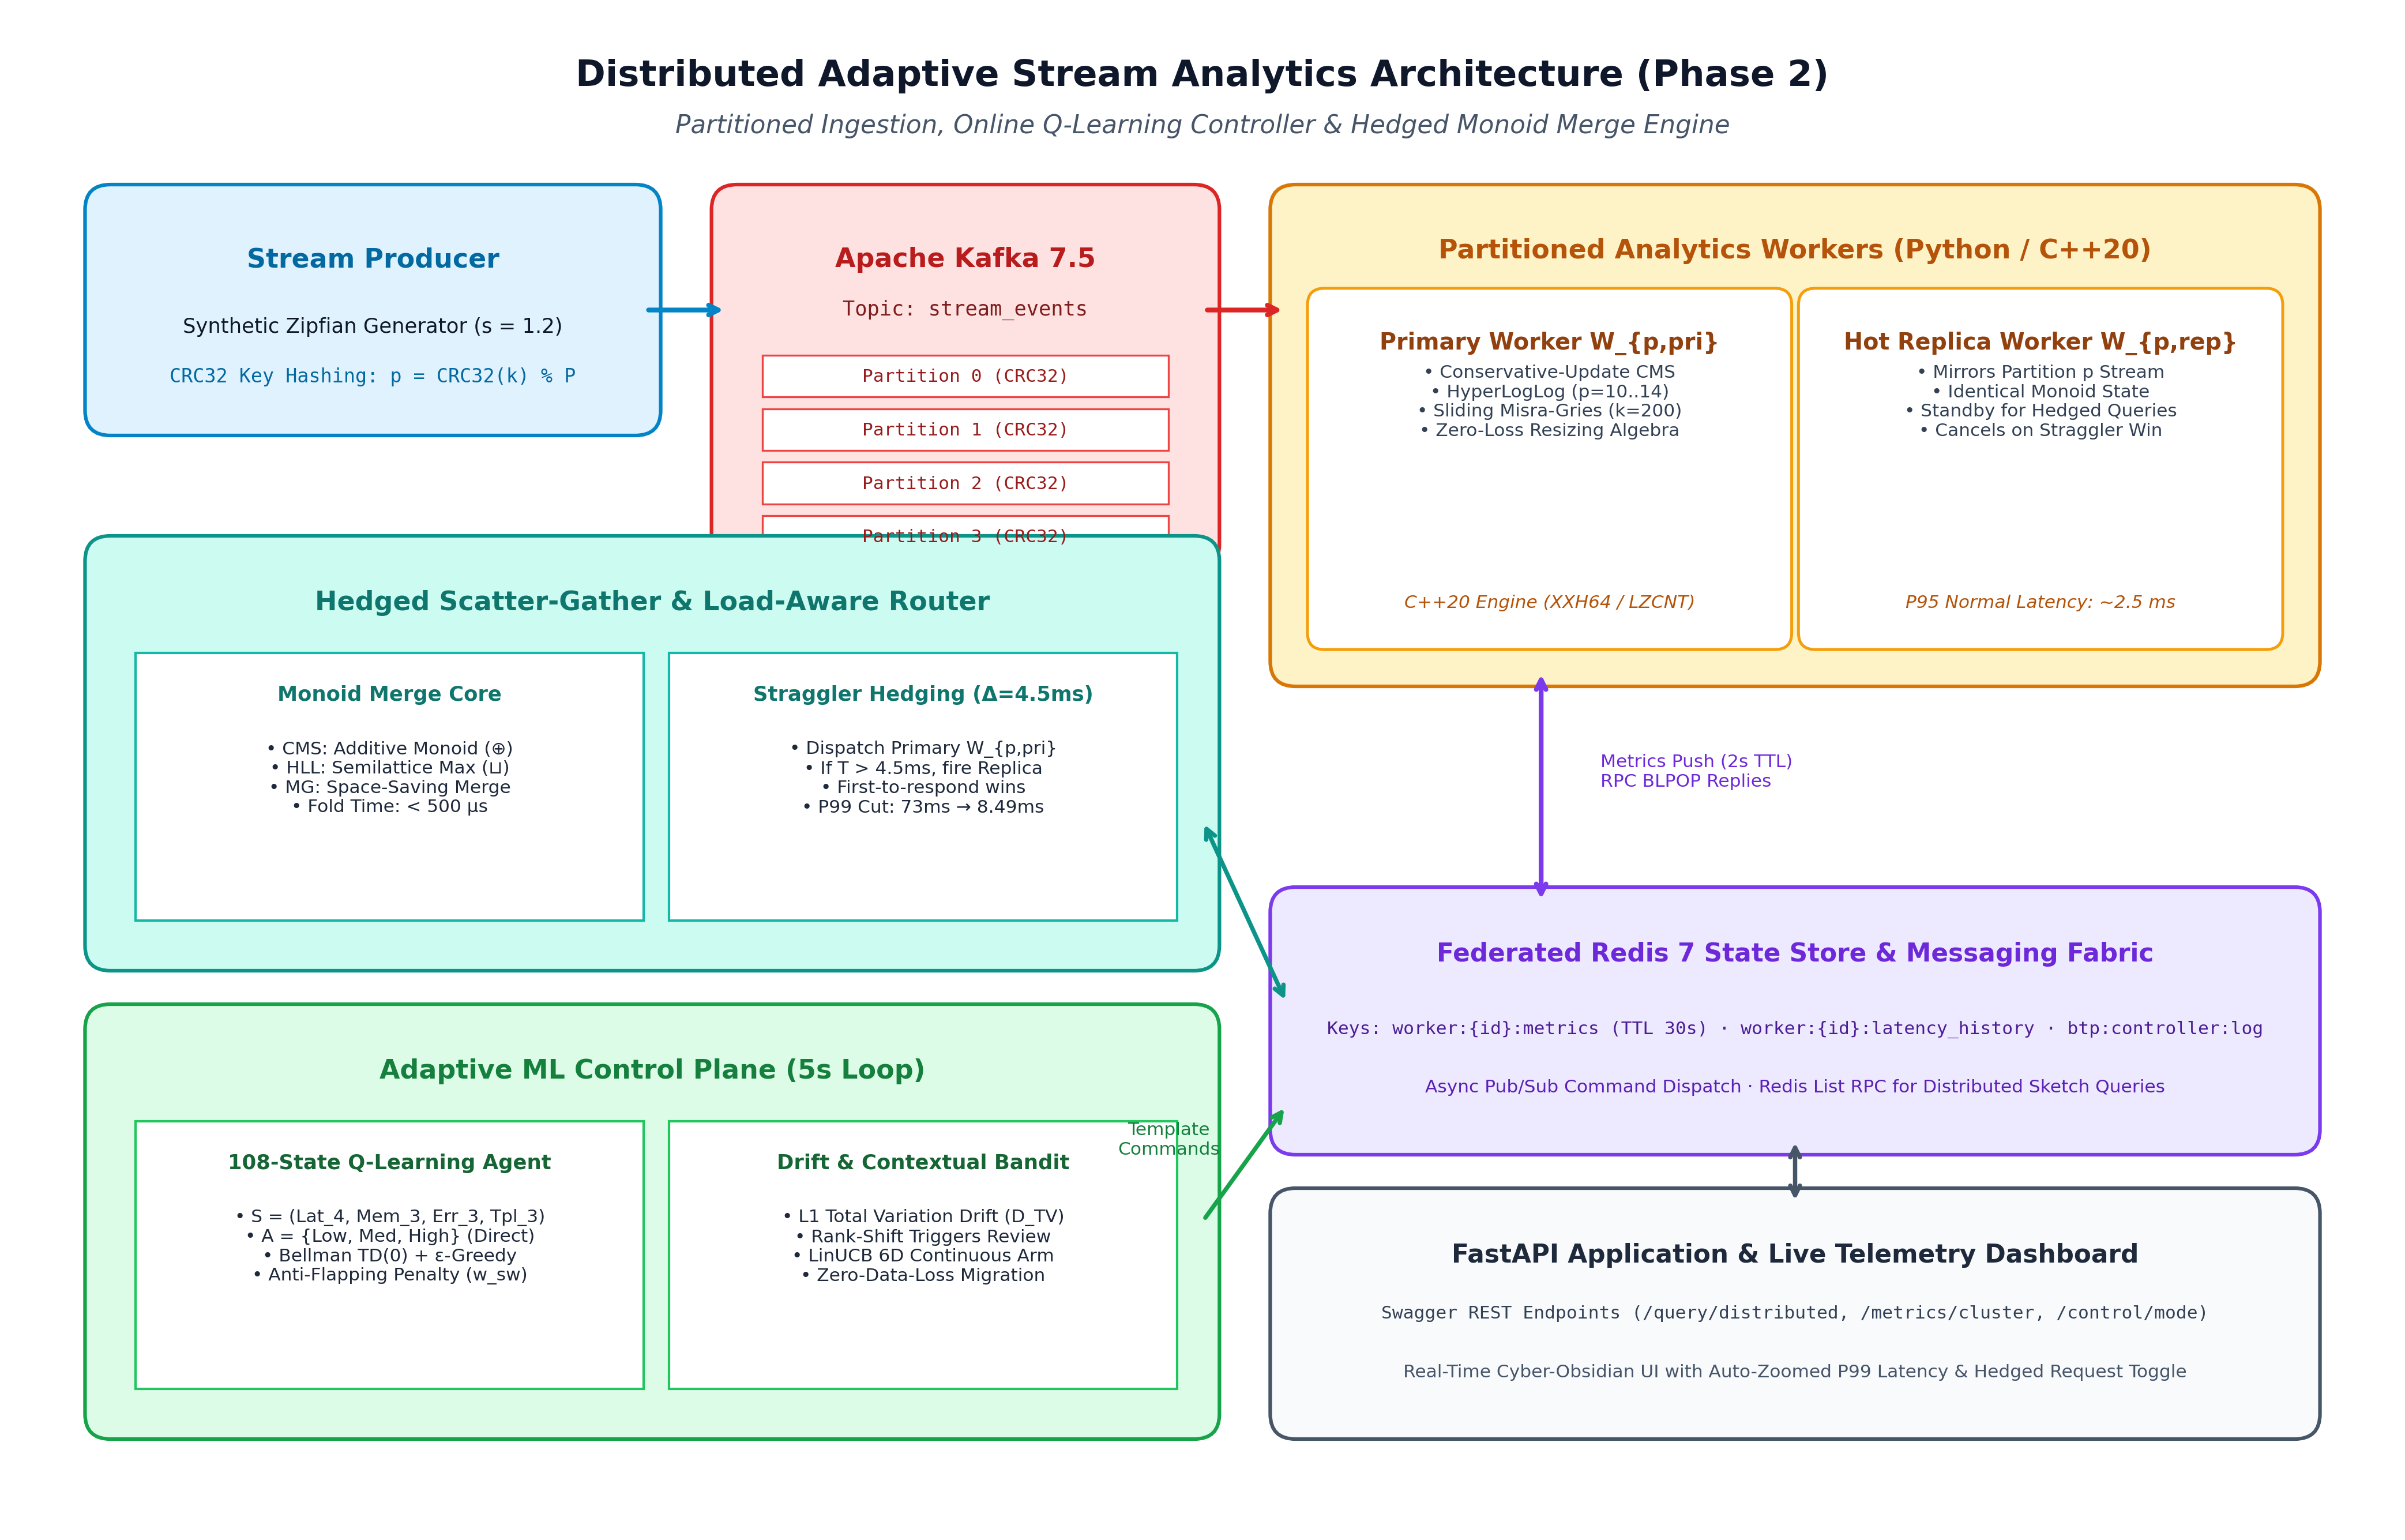
\includegraphics[width=0.95\textwidth]{Figures/architecture_diagram.png}
 \caption{End-to-end distributed system architecture. The pipeline integrates a Zipfian stream producer, a partitioned Kafka messaging backbone, dual-language analytical worker nodes (Python and C++20), an in-memory Redis telemetry blackboard, an asynchronous FastAPI query router with hedged scatter-gather execution, and an online Reinforcement Learning control plane.}
 \label{fig:arch_diagram}
\end{figure}

The platform comprises six principal architectural layers, as depicted in Figure~\ref{fig:arch_diagram}:
\begin{enumerate}
 \item \textbf{Stream Ingestion and Partitioning Layer:} A multi-threaded synthetic event producer capable of generating highly skewed, non-stationary streams governed by power-law (Zipfian) distributions, published into partitioned Kafka topics.
 \item \textbf{Decoupled Event Transport Backbone:} An Apache Kafka cluster providing partition-level log persistence, decoupled buffering, and backpressure isolation between stream producers and analytical consumers.
 \item \textbf{Heterogeneous Analytical Worker Nodes:} Autonomous worker instances implemented in Python and modern C++20 that ingest partitioned streams, execute constant-time sketch updates, collect local operating metrics, and expose live state.
 \item \textbf{Federated Telemetry and Coordination Store:} A Redis in-memory key-value store acting as a real-time blackboard for worker heartbeat telemetry, latency histograms, sketch error tracking, and controller actuation commands.
 \item \textbf{Load-Aware Routing and Scatter-Gather Query Plane:} An asynchronous FastAPI service that resolves point queries via utility-scored routing and resolves global cluster-wide aggregate queries via Monoid-based scatter-gather merges with latency hedging.
 \item \textbf{Online Machine Learning Control Plane:} An autonomous control agent implementing tabular Q-Learning over a 108-state discrete Markov Decision Process (with a continuous LinUCB contextual bandit comparator) to dynamically adapt worker sketch precision templates under varying workloads.
\end{enumerate}

\section{Stream Ingestion and Partitioning Engine}

\subsection{Zipfian Traffic Modeling and Non-Stationary Dynamics}
Real-world network telemetry, search engine queries, and e-commerce access logs exhibit pronounced skewness, wherein a tiny minority of unique keys accounts for the vast majority of event occurrences~\cite{zipf}. To evaluate the system under realistic operational stress, the ingestion pipeline generates synthetic events adhering to a discrete Zipf-Mandelbrot probability mass function:
\begin{equation}
    P(X = k) = \frac{1 / (k + q)^s}{\sum_{n=1}^N 1 / (n + q)^s}
\end{equation}
where $k \in \{1, 2, \dots, N\}$ denotes the key rank within a vocabulary of size $N$, $s$ represents the power-law exponent (default $s = 1.2$), and $q \ge 0$ is a rank-flattening parameter. Each generated record is framed as a lightweight JSON document containing the key identifier and a microsecond-resolution wall-clock timestamp:
\begin{lstlisting}[language=Python, caption=Schema of stream events published to Kafka.]
{"key": "item_42", "ts": 1710000000.123456}
\end{lstlisting}

To simulate non-stationary streaming environments and evaluate adaptive mechanisms, the ingestion generator incorporates automated concept drift. At configurable time intervals $\Delta t_{\text{shift}}$ (invoked via \texttt{--shift-interval}), the generator permutes key rankings by swapping the identity of the top-ranked item with a randomly chosen item from the distribution's long tail. This abrupt shift forces streaming models to detect distribution changes and adapt their internal state structures.

\subsection{Partition Topology and Kafka Message Transport}
The message bus relies on Apache Kafka~\cite{kafka} to decouple high-volume ingestion from downstream processing. Key partitioning strategies and transport characteristics include:
\begin{itemize}
 \item \textbf{Deterministic Partition Hashing:} In partitioned cluster topologies, events are dispatched across $P$ Kafka partitions using deterministic key hashing:
 \begin{equation}
        p = \text{CRC32}(k) \pmod P
    \end{equation}
 This ensures that all occurrences of a specific key $k$ map consistently to partition $p$, enabling exact partitioning of the underlying stream support.
 \item \textbf{Consumer Group Fanout vs. Partitioned Worker Sharding:} The platform supports two operational modes: (i) an \textit{analytics fan-out mode}, where each worker joins an independent consumer group and ingests the full stream (useful for benchmarking heterogeneous worker implementations), and (ii) a \textit{partitioned sharded mode}, where worker groups coordinate to process disjoint partitions in parallel.
 \item \textbf{Offset-Based Backpressure Management:} Ingestion workers maintain independent consumer offsets, ensuring zero data loss during transient CPU stalls, memory pressure, or in-flight sketch reallocations.
\end{itemize}

\section{Analytical Worker Design}

Each analytical worker runs as an independent OS process, maintaining local, in-memory instances of the three core probabilistic sketches: Count-Min Sketch with Conservative Updating, HyperLogLog, and Sliding-Window Misra--Gries. Workers periodically flush operational telemetry to Redis and listen for remote template reconfiguration commands.

\subsection{Python Analytical Worker}
The reference Python worker is built on an asynchronous event loop utilizing \texttt{kafka-python-ng} for stream ingestion. Hashing operations utilize MurmurHash3 (\texttt{mmh3}) and MD5 digests truncated to 64-bit integer seeds. Key characteristics include:
\begin{itemize}
 \item \textbf{Synchronous Processing Hot Path:} Incoming message batches are decoded and dispatched sequentially to sketch data structures in memory.
 \item \textbf{Windowed Latency Profiling:} Worker telemetry tracks update latencies using a rolling circular buffer of the most recent 500 operations, computing the empirical 95th and 99th percentile latencies ($P95$ and $P99$).
 \item \textbf{Resource Monitoring:} Host-level resource consumption (CPU utilization percentage and resident memory footprint) is collected every 2 seconds via \texttt{psutil}.
 \item \textbf{RPC In-Memory Response Engine:} In addition to streaming ingestion, workers maintain a dedicated Redis-based command listener that processes direct RPC query requests for live point frequency lookups.
\end{itemize}

\subsection{High-Performance C++20 Analytical Worker}
To establish the maximum single-node processing throughput, a drop-in C++20 worker was developed using identical Kafka topic configurations and Redis key schemas. The C++ implementation achieves approximately an order of magnitude higher update rates through several low-level optimizations:
\begin{itemize}
 \item \textbf{Hardware-Optimized xxHash (XXH64):} The C++ worker replaces general-purpose hashing with \texttt{XXH64}, an ultra-fast non-cryptographic hash algorithm executing at near-RAM memory bus speeds ($>13\text{ GB/s}$), providing a $\sim 10\times$ throughput improvement over standard MD5/SHA algorithms.
 \item \textbf{Single-Cycle Bit Manipulation Intrinsics:} In the HyperLogLog register update path, leading-zero counting is implemented using C++20's \texttt{std::countl\_zero()}, which the compiler translates directly into hardware-accelerated CPU instructions (\texttt{LZCNT} on x86-64 or \texttt{CLZ} on ARM64), eliminating software loop overhead.
 \item \textbf{Concurrency Without GIL Penalties:} Read-write synchronization utilizes \texttt{std::shared\_mutex}, allowing concurrent query reads via shared reader locks without contending with streaming update writers. This eliminates the Global Interpreter Lock (GIL) bottlenecks present in CPython.
\end{itemize}

\section{Federated Telemetry and State Management}

Redis~\cite{redis} serves as the centralized communication blackboard connecting analytical workers, the query routing engine, the ML controller, and the web frontend. The Redis namespace is partitioned according to the schema detailed in Table~\ref{tab:redis_keys}.

\begin{table}[htbp]
\centering
\begin{tabular}{l l l l}
\toprule
\textbf{Key Pattern} & \textbf{Data Structure} & \textbf{Producer} & \textbf{Consumer} \\
\midrule
\texttt{worker:\{id\}:metrics}        & Hash / JSON & Analytical Worker & Router, Controller, API \\
\texttt{worker:\{id\}:latency\_hist}  & List (FIFO) & Analytical Worker & Web Dashboard \\
\texttt{worker:\{id\}:cmd}            & Pub/Sub Channel & Controller & Analytical Worker \\
\texttt{controller:log}               & List (Capped) & ML Controller & Web Dashboard \\
\texttt{router:query\_log}            & List (Capped) & Query Router & Web Dashboard \\
\texttt{cluster:topology}             & Set & Discovery Module & Query Router \\
\bottomrule
\end{tabular}
\caption{Redis telemetry and command key schema.}
\label{tab:redis_keys}
\end{table}

All worker telemetry keys are configured with a strict 30-second Time-To-Live (TTL). If an analytical node experiences a fatal crash or network partition, its heartbeat expires automatically, causing the routing plane and controller to immediately drop the failed worker from routing consideration without requiring external cluster fencing.

\section{Load-Aware Request Routing Engine}

Standard stream processing architectures typically dispatch incoming analytics queries across nodes using unweighted Round-Robin or random load balancing. However, in heterogeneous or dynamically adapting clusters, workers operate with differing sketch precision templates, latency profiles, and memory pressures. Dispatching queries to a worker undergoing memory saturation or high latency degrades system reliability.

To address this, we developed a multi-criteria \textbf{Utility Scoring Router}. For each active worker $i \in \{1, \dots, W\}$, the router retrieves its latest telemetry from Redis and evaluates an operational utility score $S_i(t) \in [0, 1]$:
\begin{equation}
    S_i(t) = w_{\text{lat}} \cdot \mathcal{N}_{\text{lat}}(\text{P99}_i) + w_{\text{mem}} \cdot (1.0 - U_{\text{mem}, i}) + w_{\text{err}} \cdot (1.0 - \min(1.0, 10 \cdot \hat{\epsilon}_i))
    \label{eq:node_score}
\end{equation}
where:
\begin{itemize}
 \item $\mathcal{N}_{\text{lat}}(\text{P99}_i) = \max\left(0.0, 1.0 - \frac{\text{P99}_i}{\text{SLA}_{\text{lat}}}\right)$ evaluates normalized latency headroom against the operational SLA limit ($\text{SLA}_{\text{lat}} = 20.0\text{ ms}$).
 \item $U_{\text{mem}, i} \in [0, 1]$ represents the fraction of host memory currently utilized.
 \item $\hat{\epsilon}_i$ represents the empirical Weighted Absolute Percentage Error (WAPE) of the worker's Count-Min Sketch.
 \item $w_{\text{lat}}, w_{\text{mem}}, w_{\text{err}} \ge 0$ are weighting coefficients satisfying $w_{\text{lat}} + w_{\text{mem}} + w_{\text{err}} = 1.0$ (configured by default to $0.4, 0.3, 0.3$).
\end{itemize}

\subsection{Routing Policies}
The router supports two operational selection regimes:
\begin{enumerate}
 \item \textbf{Deterministic Greedy Routing:} The router dispatches the incoming query to the worker exhibiting the highest instantaneous utility score:
 \begin{equation}
        i^* = \arg\max_{i \in \mathcal{W}_{\text{active}}} S_i(t)
    \end{equation}
 \item \textbf{Boltzmann Softmax Routing:} To prevent herd behavior and distribute load across healthy replicas, queries can be routed probabilistically according to a Gibbs distribution:
 \begin{equation}
        P(\text{Route to Worker } i) = \frac{\exp(S_i(t) / \tau)}{\sum_{j \in \mathcal{W}_{\text{active}}} \exp(S_j(t) / \tau)}
    \end{equation}
 where $\tau > 0$ denotes a temperature parameter governing exploration spread.
\end{enumerate}

\section{Online Machine Learning Controller}

Fixed heuristic controllers relying on static thresholds suffer from policy flapping, poor stability under multi-regime traffic bursts, and inability to balance conflicting operational objectives (e.g., maintaining low query error while strictly obeying memory and latency limits). In Phase~2, we formulated the dynamic sketch parameter tuning problem as an online Reinforcement Learning task.

\subsection{108-State Discrete Markov Decision Process (MDP)}
We model the adaptive control plane as a discrete-time Markov Decision Process defined by the tuple $\langle \mathcal{S}, \mathcal{A}, \mathcal{P}, \mathcal{R}, \gamma \rangle$:

\begin{itemize}
 \item \textbf{State Space $\mathcal{S}$ ($|\mathcal{S}| = 108$):} Each worker's operating state $s_t \in \mathcal{S}$ is characterized by four discrete dimensions:
 \begin{equation}
        s_t = \langle L_t, M_t, E_t, T_t \rangle
    \end{equation}
 where:
 \begin{enumerate}
 \item \textbf{Latency Bin $L_t \in \{0, 1, 2, 3\}$:} Captures worker update latency with a proactive warning threshold:
 \begin{itemize}
 \item $0$ (Normal): $\text{P99} < 10.0\text{ ms}$
 \item $1$ (Elevated): $10.0\text{ ms} \le \text{P99} < 14.0\text{ ms}$
 \item $2$ (Proactive Approaching-SLA): $14.0\text{ ms} \le \text{P99} < 20.0\text{ ms}$ (representing $70\%\text{--}100\%$ of SLA)
 \item $3$ (SLA Violated): $\text{P99} \ge 20.0\text{ ms}$
 \end{itemize}
 \item \textbf{Memory Bin $M_t \in \{0, 1, 2\}$:}
 \begin{itemize}
 \item $0$ (Low): Memory usage $< 60\%$
 \item $1$ (Moderate): $60\% \le \text{Memory} < 80\%$
 \item $2$ (High/Critical): $\text{Memory} \ge 80\%$
 \end{itemize}
 \item \textbf{Empirical Error Bin $E_t \in \{0, 1, 2\}$:}
 \begin{itemize}
 \item $0$ (Low Error): $\hat{\epsilon}_{\text{WAPE}} < 1.0\%$
 \item $1$ (Moderate Error): $1.0\% \le \hat{\epsilon}_{\text{WAPE}} < 3.0\%$
 \item $2$ (High Error): $\hat{\epsilon}_{\text{WAPE}} \ge 3.0\%$
 \end{itemize}
 \item \textbf{Active Template Bin $T_t \in \{0, 1, 2\}$:} Represents the worker's current sketch configuration template ($\text{Low} = 0$, $\text{Medium} = 1$, $\text{High} = 2$).
 \end{enumerate}
 The total number of unique states is given by:
 \begin{equation}
        |\mathcal{S}| = |L| \times |M| \times |E| \times |T| = 4 \times 3 \times 3 \times 3 = 108 \text{ states}
    \end{equation}

 \item \textbf{Action Space $\mathcal{A}$ ($|\mathcal{A}| = 3$):} The action represents the target sketch template directly:
 \begin{equation}
        \mathcal{A} = \{\text{Low}, \text{Medium}, \text{High}\}
    \end{equation}
 Direct action assignment enables single-step jump capability. Under severe latency or memory spikes, the controller can transition directly from $\text{High}$ to $\text{Low}$ in a single decision cycle rather than stepping through intermediate states.

 \item \textbf{Reward Function $\mathcal{R}$:} The composite reward function $R_t \in [-1, 1]$ balances multiple competing objectives:
 \begin{equation}
        R_t = 1.0 - \left(w_e \cdot C_{\text{err}} + w_l \cdot C_{\text{lat}} + w_m \cdot C_{\text{mem}} + w_s \cdot \mathbb{I}[a_t \ne T_t]\right) + B_{\text{prec}}
        \label{eq:rl_reward}
    \end{equation}
 where:
 \begin{itemize}
 \item $C_{\text{err}} = \min(1.0, 10.0 \cdot \hat{\epsilon}_{\text{WAPE}})$ penalizes empirical estimation error.
 \item $C_{\text{lat}}$ implements a nonlinear hinge penalty for latency violations:
 \begin{equation}
            C_{\text{lat}} = \begin{cases}
                \frac{\text{P99}}{20.0} & \text{if } \text{P99} \le 20.0\text{ ms} \\
                1.0 + 2.0 \cdot \left(\frac{\text{P99} - 20.0}{20.0}\right) & \text{if } \text{P99} > 20.0\text{ ms}
            \end{cases}
        \end{equation}
 \item $C_{\text{mem}}$ penalizes memory pressure, ramping up sharply above $80\%$:
 \begin{equation}
            C_{\text{mem}} = \begin{cases}
                \frac{U_{\text{mem}}}{0.80} & \text{if } U_{\text{mem}} \le 0.80 \\
                1.0 + 3.0 \cdot (U_{\text{mem}} - 0.80) & \text{if } U_{\text{mem}} > 0.80
            \end{cases}
        \end{equation}
 \item $w_s \cdot \mathbb{I}[a_t \ne T_t]$ represents an anti-flapping switching penalty ($w_s = 0.15$), penalizing unnecessary template transitions.
 \item $B_{\text{prec}} \in \{0.0, 0.05, 0.10\}$ provides a small positive bonus for sustaining higher precision templates when resource headroom permits.
 \end{itemize}
\end{itemize}

\subsection{Temporal Difference Q-Learning Formulation}
The agent learns an optimal action-value function $Q^*(s, a)$ online via tabular Temporal Difference (TD(0)) updates:
\begin{equation}
    Q(s_t, a_t) \leftarrow Q(s_t, a_t) + \alpha \left[ R_{t+1} + \gamma \max_{a' \in \mathcal{A}} Q(s_{t+1}, a') - Q(s_t, a_t) \right]
\end{equation}
where $\alpha \in (0, 1]$ is the learning rate (default $\alpha = 0.1$) and $\gamma \in [0, 1)$ is the discount factor (default $\gamma = 0.85$). 

Exploration is managed via an $\epsilon$-greedy schedule with exponential decay:
\begin{equation}
    \epsilon_k = \max\left(\epsilon_{\min},\; \epsilon_0 \cdot d^k\right)
\end{equation}
where $\epsilon_0 = 1.0$, $d = 0.98$, and $\epsilon_{\min} = 0.05$. The learned $Q$-table is periodically serialized to JSON, enabling persistent policy reuse across system restarts.

\subsection{Continuous-Feature LinUCB Contextual Bandit Comparator}
As an algorithmic baseline to evaluate whether multi-step sequential lookahead ($\gamma > 0$) is necessary over myopic continuous-feature optimization ($\gamma = 0$), we implemented a disjoint **Linear Upper Confidence Bound (LinUCB)** contextual bandit agent~\cite{li2010contextual}.

For each decision round $t$, the LinUCB agent observes a 6-dimensional continuous context vector:
\begin{equation}
    \mathbf{x}_t = \begin{bmatrix} 1.0, & \frac{\text{P99}_t}{20.0}, & \frac{U_{\text{mem}, t}}{100.0}, & \frac{\hat{\epsilon}_{\text{WAPE}, t}}{0.05}, & D_{\text{TV}, t}, & \frac{T_t}{2.0} \end{bmatrix}^\top \in \mathbb{R}^6
\end{equation}
For each discrete arm $a \in \{\text{Low}, \text{Med}, \text{High}\}$, the agent maintains a ridge-regression covariance matrix $\mathbf{A}_a \in \mathbb{R}^{6 \times 6}$ (initialized to $\mathbf{I}_6$) and response vector $\mathbf{b}_a \in \mathbb{R}^6$ (initialized to $\mathbf{0}$). The ridge regression weight estimate is computed as:
\begin{equation}
    \hat{\boldsymbol{\theta}}_a = \mathbf{A}_a^{-1} \mathbf{b}_a
\end{equation}
The agent selects the template arm maximizing the upper confidence bound:
\begin{equation}
    a_t = \arg\max_{a \in \mathcal{A}} \left[ \hat{\boldsymbol{\theta}}_a^\top \mathbf{x}_t + \alpha_{\text{ucb}} \sqrt{\mathbf{x}_t^\top \mathbf{A}_a^{-1} \mathbf{x}_t} \right]
\end{equation}
Upon observing the scalar environment reward $R_t$ (Eq.~\ref{eq:rl_reward}), the selected arm's parameters are updated via rank-1 online updates:
\begin{align}
    \mathbf{A}_{a_t} &\leftarrow \mathbf{A}_{a_t} + \mathbf{x}_t \mathbf{x}_t^\top \\
    \mathbf{b}_{a_t} &\leftarrow \mathbf{b}_{a_t} + R_t \mathbf{x}_t
\end{align}

\section{Concept Drift Detection Engine}

In streaming data architectures, input key distributions often undergo sudden changes. If a learning controller assumes stationarity, its learned policy may persist with sub-optimal sketch allocations. To provide automated drift sensitivity, the platform incorporates an $L_1$ Total Variation Distance ($D_{\text{TV}}$) drift detector operating over sliding Misra--Gries snapshots.

Let $\mathcal{K}_t$ and $\mathcal{K}_{t-1}$ represent the sets of heavy-hitter keys identified in the current and preceding sliding windows, and let $p_t(k)$ denote the empirical relative frequency of key $k$ in window $t$. The Total Variation Distance between consecutive distributions is defined as:
\begin{equation}
    D_{\text{TV}}(P_t, P_{t-1}) = \frac{1}{2} \sum_{k \in \mathcal{K}_t \cup \mathcal{K}_{t-1}} |p_t(k) - p_{t-1}(k)| \in [0, 1]
    \label{eq:drift_formula}
\end{equation}
A drift alert is triggered whenever $D_{\text{TV}}(P_t, P_{t-1}) > \tau_{\text{drift}}$ (default $\tau_{\text{drift}} = 0.15$). When drift is detected:
\begin{enumerate}
 \item The telemetry blackboard registers an active concept drift event.
 \item The Q-Learning agent temporarily boosts its exploration parameter $\epsilon \leftarrow \max(\epsilon, 0.30)$, accelerating policy re-adaptation to the newly emerged heavy-hitter distribution.
 \item Telemetry logs record the exact shift magnitude for post-mortem auditing.
\end{enumerate}

\section{Zero-Data-Loss Dynamic Sketch Resizing Algebra}

A major vulnerability in naive adaptive streaming systems is that altering sketch dimensions during runtime typically requires discarding the existing sketch and allocating an empty matrix, discarding all historical state accumulated up to that point. In Phase~2, we developed a **Zero-Data-Loss Sketch Resizing Algebra** that enables dynamic resizing without dropping counts.

\subsection{Count-Min Sketch Downscaling via Modular Hash Folding}
Let $C_1 \in \mathbb{N}^{d \times w_1}$ be an active Count-Min Sketch matrix with width $w_1 = 2^{k_1}$, utilizing hash functions $h_i(x) \pmod{w_1}$ for row $i \in \{1, \dots, d\}$. When downscaling to a smaller template with width $w_2 = 2^{k_2}$ where $w_2 < w_1$ and $w_1 = m \cdot w_2$ ($m \in \mathbb{N}$ is a power of 2), we fold the columns of each row into the new matrix $C_2 \in \mathbb{N}^{d \times w_2}$ according to modular arithmetic:
\begin{equation}
    C_2[i, j'] = \sum_{r=0}^{m-1} C_1[i, j' + r \cdot w_2] \quad \forall j' \in \{0, \dots, w_2-1\}
    \label{eq:cms_folding}
\end{equation}

\paragraph{Theorem 1 (Preservation of the No-Undercount Invariant):}
\textit{Under modular hash folding (Eq.~\ref{eq:cms_folding}), the folded sketch $C_2$ never undercounts any stream element; that is, for all items $x$, $\hat{f}_{C_2}(x) \ge f_{\text{true}}(x)$.}

\paragraph{Proof:}
For any key $x$, its hash bucket in the original matrix $C_1$ is $j_1 = h_i(x) \pmod{w_1}$. In the resized matrix $C_2$, the hash bucket is $j_2 = h_i(x) \pmod{w_2}$. Because $w_1$ is an integer multiple of $w_2$, modular congruence dictates:
\begin{equation}
    j_1 \pmod{w_2} = (h_i(x) \pmod{w_1}) \pmod{w_2} = h_i(x) \pmod{w_2} = j_2
\end{equation}
Therefore, the original bucket $j_1$ is one of the $m$ terms summed into $C_2[i, j_2]$ in Eq.~\ref{eq:cms_folding}. Because all entries in $C_1$ are non-negative ($C_1 \ge 0$), we have:
\begin{equation}
    C_2[i, j_2] = C_1[i, j_1] + \sum_{r \ne r^*} C_1[i, j_2 + r \cdot w_2] \ge C_1[i, j_1] \ge f_{\text{true}}(x)
\end{equation}
Taking the minimum over all $d$ rows confirms that $\hat{f}_{C_2}(x) = \min_i C_2[i, h_i(x) \pmod{w_2}] \ge f_{\text{true}}(x)$. The no-undercount guarantee is rigorously preserved. $\blacksquare$

\subsection{HyperLogLog Downscaling via Register Max-Folding}
When transitioning HyperLogLog cardinality sketches from precision $p_1$ (with $m_1 = 2^{p_1}$ registers) to a lower precision $p_2 < p_1$ (with $m_2 = 2^{p_2}$ registers), we map the registers by taking the coordinate-wise maximum:
\begin{equation}
    R_2[j'] = \max_{r \in \{0, \dots, 2^{p_1 - p_2} - 1\}} R_1[j' + r \cdot m_2] \quad \forall j' \in \{0, \dots, m_2 - 1\}
\end{equation}
This operation preserves the most extreme leading-zero observations made across all folded sub-registers, ensuring that cardinality estimates remain monotonically consistent without catastrophic reset.

\subsection{Safe Upscaling Protocol}
When scaling up from a smaller template to a larger template ($w_2 > w_1$), historical counts cannot be unfolded deterministically because hash information has already been compressed. The worker resolves this by instantiating the new matrix $C_{\text{new}}$ initialized to zero, while retaining the old folded matrix $C_{\text{old}}$ as a fallback baseline. For any query during the transition window, the point estimate is answered as:
\begin{equation}
    \hat{f}(x) = \hat{f}_{C_{\text{new}}}(x) + \hat{f}_{C_{\text{old}}}(x)
\end{equation}
Once the new sketch accumulates sufficient operational mass, $C_{\text{old}}$ is safely reclaimed by the runtime memory manager.

\section{Partitioned Ingestion and Hedged Monoid Merge Plane}
\label{sec:hedged_monoid_arch}

While single-stream fanout architectures suffice for moderate workloads, horizontally scaling write throughput to millions of events per second requires stream partitioning. However, distributed scatter-gather queries over partitioned sketches face the straggler problem, where overall latency is bounded by the slowest responder. Phase~2 resolves this via a distributed **Partitioned Ingestion Engine with Hedged Monoid Merges**.

\subsection{Monoid Merge Algebra for Distributed Aggregation}
Probabilistic summary structures form algebraic \textbf{Monoids} $(\mathcal{S}, \oplus, \mathbf{0})$ governed by an associative binary operator $\oplus$ and identity element $\mathbf{0}$:
\begin{align}
    (A \oplus B) \oplus C &= A \oplus (B \oplus C) \quad &&\text{(Associativity)} \\
    A \oplus \mathbf{0} &= \mathbf{0} \oplus A = A \quad &&\text{(Identity)}
\end{align}
Because disjoint partitions process independent subsets of the global stream, global queries do not require raw event transmission. Instead, workers transmit compact partial sketch matrices ($\sim 50\text{--}100\text{ KB}$), which the query coordinator merges in $<500\ \mu\text{s}$:

\begin{enumerate}
 \item \textbf{Count-Min Sketch (Element-Wise Addition):}
 Let $\mathbf{C}_p \in \mathbb{N}^{d \times w}$ be the count matrix on partition $p \in \{0, \dots, P-1\}$. The cluster-wide merged sketch is computed as:
 \begin{equation}
        \mathbf{C}_{\text{global}}[i, j] = \sum_{p=0}^{P-1} \mathbf{C}_p[i, j] \quad \forall i \in [d], j \in [w]
    \end{equation}
 Because matrix addition over $\mathbb{N}$ is associative and commutative, CMS forms an Abelian Monoid. The global point estimate satisfies $\hat{f}(x) \le f_{\text{global}}(x) + \frac{e}{w} \sum_p N_p$.

 \item \textbf{HyperLogLog (Coordinate-Wise Join Semilattice):}
 Let $\mathbf{R}_p \in \mathbb{N}^m$ be the register array of partition $p$. The merged cluster register array is:
 \begin{equation}
        \mathbf{R}_{\text{global}}[i] = \max_{p \in \{0, \dots, P-1\}} \mathbf{R}_p[i] \quad \forall i \in \{0, \dots, m-1\}
    \end{equation}
 Because $\max(a, b)$ is associative, commutative, and idempotent ($\max(a, a) = a$), HyperLogLog forms a bounded join-semilattice. Even under duplicate event delivery across partitions, register max-folding preserves exact deduplicated union cardinality.

 \item \textbf{Misra--Gries (Space-Saving Monoid Merge):}
 Following Agarwal et al.~\cite{agarwal2013mergeable}, candidate heavy-hitter frequencies from all partitions are combined: $f_{\text{merged}}(x) = \sum_p f_p(x)$. If the number of unique candidate keys exceeds capacity $k = \min_p k_p$, the $k^{\text{th}}$ largest count $C_{\min}$ is subtracted from all candidate counts, retaining only items with positive remainder. The merged summary guarantees bounded additive error:
 \begin{equation}
        \text{Error Bound} \le \frac{\sum_p N_p}{\min_p k_p}
    \end{equation}
\end{enumerate}

\subsection{Straggler Mitigation via Asynchronous Hedged Requests}
In any distributed scatter-gather query over $P$ partitions, total query completion latency is governed by the slowest responding partition:
\begin{equation}
    T_{\text{query}} = \max_{p \in \{0, \dots, P-1\}} T_p
\end{equation}
If individual nodes encounter transient latency spikes (due to garbage collection pauses, OS scheduling jitter, or virtualization stalls) with probability $p_{\text{strag}} = 5\%$, the probability of a scatter-gather query stalling across $P$ partitions escalates exponentially:
\begin{equation}
    P(\text{Query Stalls}) = 1 - (1 - p_{\text{strag}})^P
\end{equation}
For $P = 4$ partitions, $18.55\%$ of all queries stall. For $P = 16$ partitions, $56.0\%$ of queries stall, causing severe tail-latency amplification.

To eliminate straggler stalls, the scatter-gather engine implements **Hedged Requests**~\cite{dean2013tail}:
\begin{enumerate}
 \item \textbf{Primary Request Dispatch:} The engine asynchronously transmits sub-queries to primary partition workers $W_{p, \text{primary}}$.
 \item \textbf{Hedge Delay Timer:} A timer is initialized to $T_{\text{hedge}}$, configured to the empirical 95th percentile latency of normal worker responses ($T_{\text{hedge}} = 4.5\text{ ms}$).
 \item \textbf{Duplicate Hedged Dispatch:} If $W_{p, \text{primary}}$ fails to respond within $T_{\text{hedge}}$, a duplicate request is immediately dispatched to hot-standby replica $W_{p, \text{replica}}$.
 \item \textbf{First-Completion Acceptance:} The engine accepts the first response to complete from either node, cancelling the outstanding task on the lagging worker.
\end{enumerate}
The effective latency for partition $p$ is bounded by:
\begin{equation}
    T_p^{\text{hedged}} = \min\left(T_{p, \text{primary}},\; T_{\text{hedge}} + T_{p, \text{replica}}\right)
\end{equation}
Because the probability of both primary and replica workers stalling simultaneously is $p_{\text{strag}}^2 = (0.05)^2 = 0.25\%$, hedged requests truncate the long tail of the latency distribution, bringing 99th percentile response times back within normal operational envelopes with less than $6\%$ network request overhead.
